\section{The Direct and Indirect Effects of Health Insurance}
\label{sec:healthinsurance}


\begin{figure}[h!]
    \caption{Effects of Health Insurance in the Oregon Health Insurance Experiment.}
    \centering
    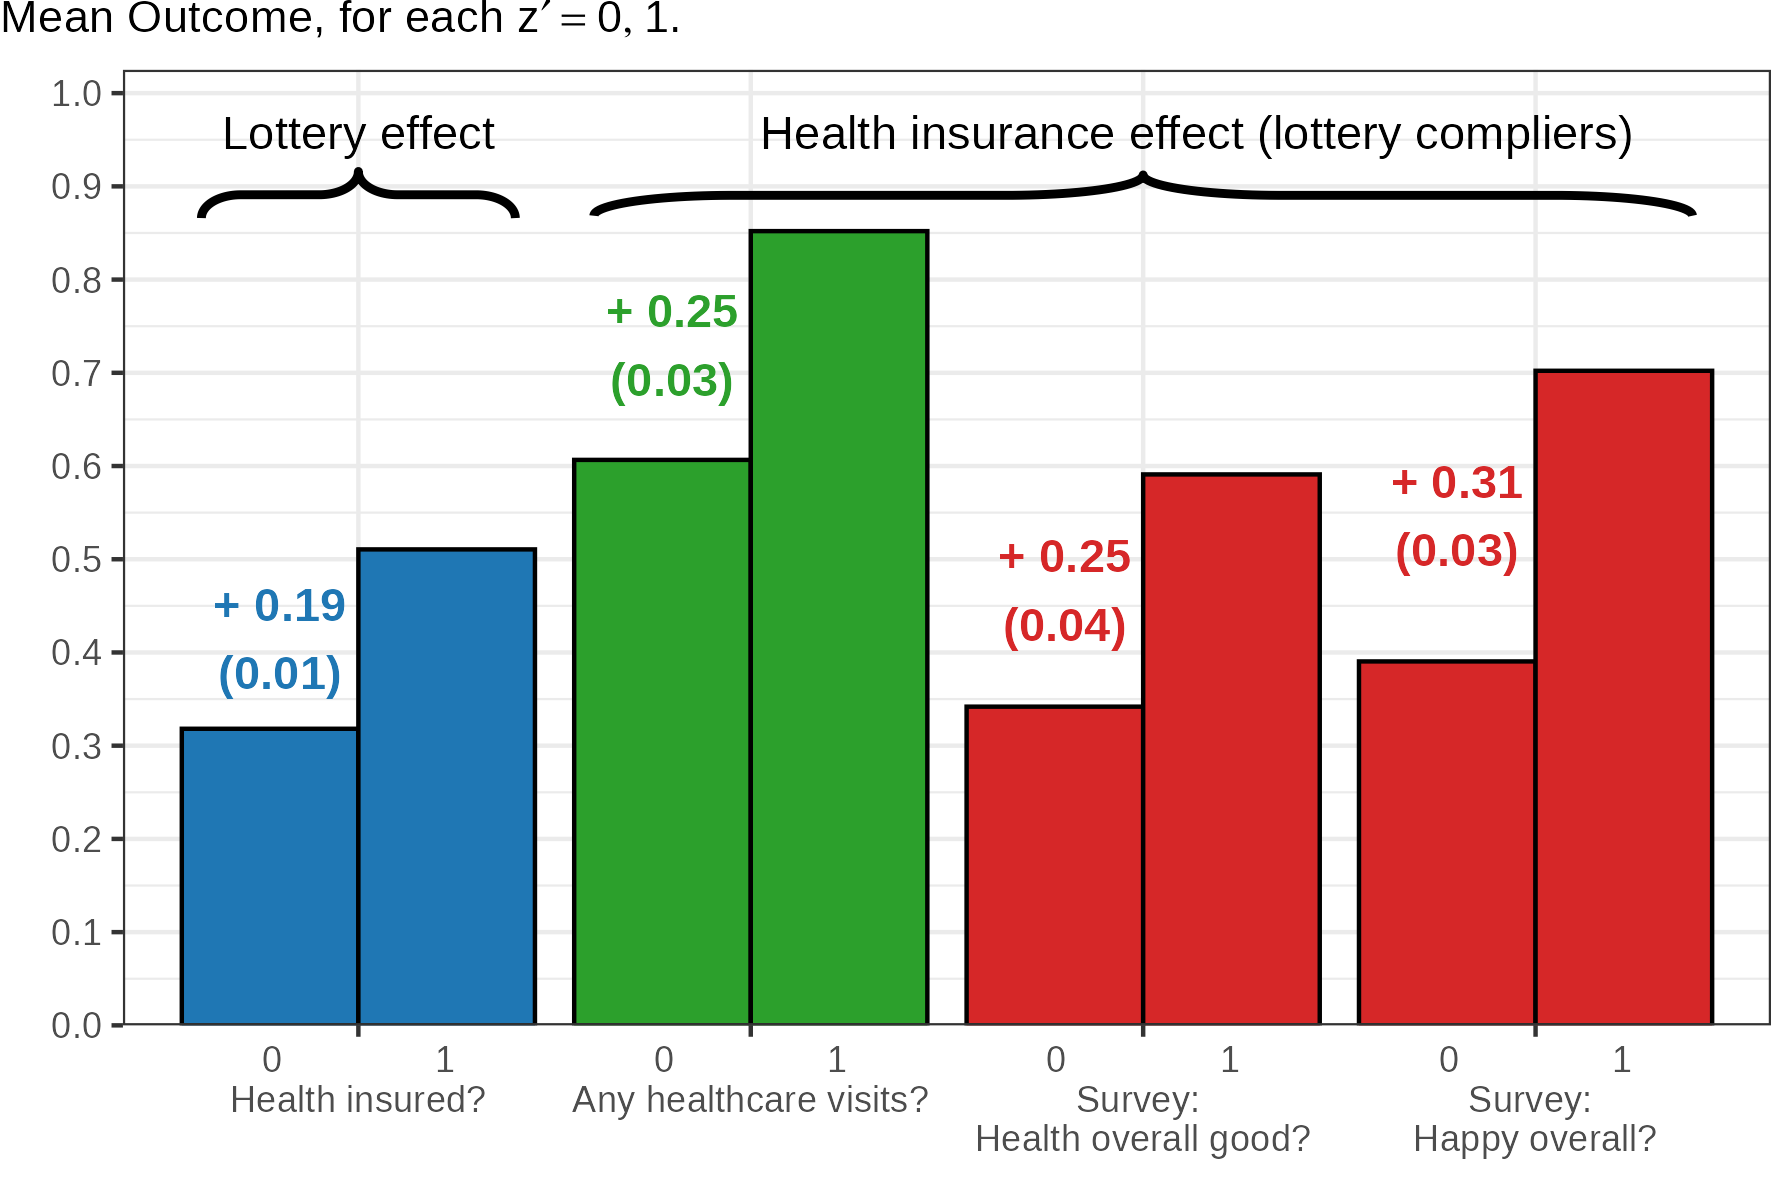
\includegraphics[width=0.85\textwidth]{sections/figures/insurance-effects.png}
    \label{fig:healthinsurance-effects}
    \justify
    \footnotesize    
    \textbf{Note:}
    This figure summarises the relevant results of the Oregon Health Insurance Experiment \citep{finkelstein2008oregon}.
    The lottery results show that being randomly selected off the Medicaid wait-list increased health insurance rate by 19 percentage points.
    The effect of health insurance shows estimates of the average complier effect of having health insurance on surveyed outcomes.
    It uses the wait-list lottery as an instrument for having health insurance, and the \cite{abadie2003semiparametric} weighting scheme to estimate the average complier levels, $\Egiven{Y_i(z',.)}{\text{lottery complier}}$ for each $z'=0,1$ with bootstrap standard errors in brackets.
\end{figure}


\subsection{Accepted Practice in Applied Economics}

Mention the Blackwell paper.
%\autoref{appendix:mediation-review}
Surveys the applied economics literature, using a databse of the NBER working paper series \citep{garg2025causalclaimseconomics}.

Writing plan:
\begin{enumerate}
    \item Take the figures from the causal claims data to show the percent of papers that claim to estimate a mediation effect, $Z \to D \to Y$
    \item Claim that they generally do so in one of two ways (1) Estimate $Z \to D, Y$ separately and then call it day\footnote{
        This is no evidence of mediation; the $D \to Y$ among $D(Z)$ compliers is assumed, with no evidence given, thus is not evidence of mechanisms.
    }
    \item Control for an intermediary variable, and call it a day; this is alluding to CM, without a clear understanding of the assumptions involved.
    \item Leave it to later to crawl the abstracts (or papers) of the claims database, saying how many papers do either.
\end{enumerate}

Until now, applied economists have assumed that mediation evidence is easy to come by, and that it can be done in any setting with random variation and valid total treatment effects.
Neither of these assumptions are true.

They have been over-claiming, and the trend is that this over-claiming will grow.


One main table, based on the review, that X\% do the assumed mechanism approach, and $Y\%$ do the controlling for mediator and getting direct effect approach.
